\chapter{Strategy}
\begin{figure}[!ht]
\begin{center}
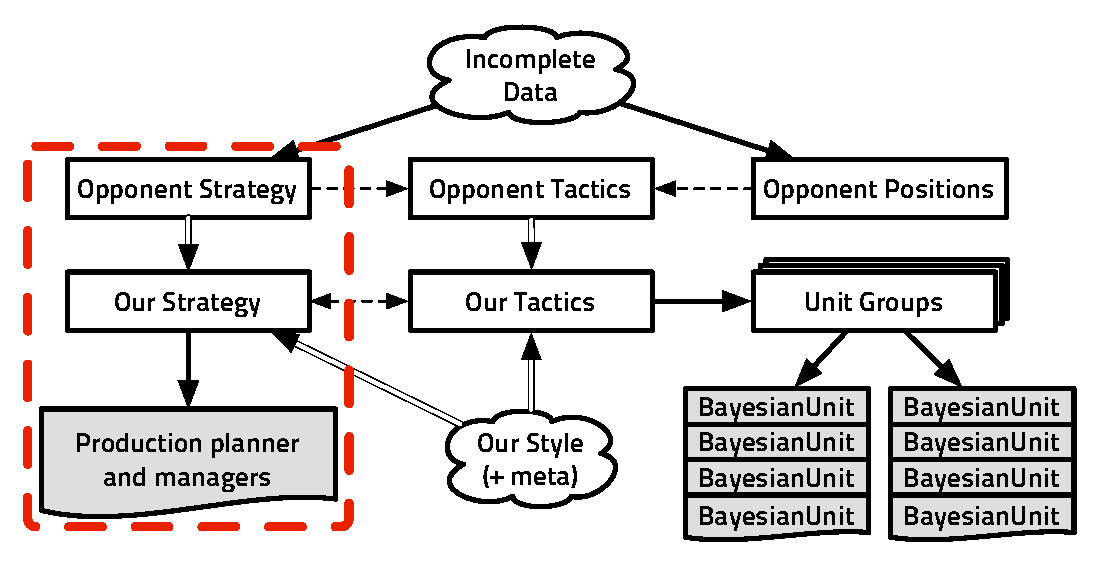
\includegraphics[width=13cm]{images/starcraft_bbq_concept_STRATEGY.pdf}
\end{center}
\label{fig:conceptSTRATEGY}
\caption{Information-centric view of the architecture of the bot, the part concerning this chapter is in the dotted rectangle}
\end{figure}
\begin{itemize}
\item Problem: take the winning strategy in the absolute
\item Complexity: without going meta, prediction is an ``inference under uncertainty'' problem, adaptation w.r.t. what we know is a planning under constraints problem. Going meta $\Rightarrow$ \texttt{(O.O)}
\item State of the art: Data mining, plan recognition, CBR... \citep{weberStrat}, \citep{Weber2010qf} and even meta \citep{metalevelbehavioradaptrts}.
\item Our take: \citep{SYNNAEVE:OpeningPred}, \citep{SYNNAEVE:StratPred}
\item Results: better resistance to noise, which is fundamental in real setup RTS gameplay (fog of war). Full Bayesian model down to adaptation actions some day?
\item Conclusion and perspectives: a way to encode and use gameplay/structural knowledge 
\end{itemize}

\section{What is a Strategy?}
% tech tree, opening, army composition, build tree

In a RTS, players need to gather resources to build military units and defeat their opponents. To that end, they often have \textit{worker units} (or extraction structures) than can gather resources needed to build \textit{workers}, \textit{buildings}, \textit{military units} and \textit{research upgrades}. Workers are often also builders (as in StarCraft) and are weak in fights compared to military units. Resources may have different uses, for instance in StarCraft: minerals are used for everything, whereas gas is only required for advanced buildings or military units, and technology upgrades. Buildings and research upgrades define technology trees (directed acyclic graphs) and each state of a ``tech tree'' allow for different unit type production abilities and unit spells/abilities. The military can be of different types, any combinations of ranged, casters, contact attack, zone attacks, big, small, slow, fast, invisible, flying... Units can have attacks and defenses that counter each others as in rock-paper-scissors. 

Each unit and building has a \textit{sight range} that provides the player with a view of the map. Parts of the map not in the sight range of the player's units are under \textit{fog of war} and the player ignores what is and happens there.
In RTS games jargon, an \newglossaryentry{opening}{name=opening,description={in Chess as in RTS games: the first strategic moves of the game, the strategy of the early game},plural=openings}\textit{\glos{opening}} denotes the same thing than in Chess: an early game plan for which the player has to make choices. In Chess because one can not move many pieces at once (each turn), in RTS games because during the development phase, one is economically limited and has to choose between economic and military priorities and can only open so many tech paths at once. The \textit{\glos{opening}} corresponds to the first military (tactical) moves that will be performed and, in StarCraft, it corresponds to the 5 (early rushes) to 15 minutes (advanced technology / late push) timespan. 
Players have to find out what opening their opponents are doing to be able to effectively deal with the strategy (army composition) and tactics (military moves: where and when) thrown at them. For that, players scout each other and reason about the incomplete information they can bring together about army and buildings composition. This paper presents a probabilistic model able to predict the \textit{\glos{opening}} of the enemy that is used in a StarCraft AI competition entry bot (see Figure~\ref{fig:}).

\section{Strategy prediction}

\subsection{Related Works}
This work was encouraged by the reading of Weber and Mateas' Data Mining Approach to Strategy Prediction \citep{weberStrat} and the fact that they provided their dataset, that we used. They tried and evaluated several machine learning algorithms on replays that were labeled with strategies (openings) with rules.


There are related works in the domains of opponent modeling \citep{HsiehS08,schadd2007opponent,OBRecog}. The main methods used to these ends are case-based reasoning (CBR) and planning or plan recognition \citep{LTW,CBR_Planning,OntanonCBR,HTNPlanning,Ramirez}. There are precedent works of Bayesian plan recognition \citep{BMPR}, even in games with Albrecht \textit{et al.} \citep{BayesianRecog} using dynamic Bayesian networks to recognize a user's plan in a multi-player dungeon adventure. 

Aha \textit{et al.} \citep{LTW} used CBR to perform dynamic plan retrieval extracted from domain knowledge in Wargus (Warcraft II clone). Onta\~{n}\'{o}n \textit{et al.} \citep{CBR_Planning} base their real-time case-based planning (CBP) system on a plan dependency graph which is learned from human demonstration. In \citep{OntanonCBR,PlanRetrieval}, they use CBR and expert demonstrations on Wargus. %They update their previous CPB approach by using ``situation assessment'' for plan retrieval. 
They improve the speed of CPB by using a decision tree to select relevant features. Hsieh and Sun \citep{HsiehS08} based their work on Aha \textit{et al.}'s CBR \citep{LTW} and used StarCraft replays to construct states and building sequences. Strategies are choices of building construction order in their model. 

Schadd \textit{et al.} \citep{schadd2007opponent} describe opponent modeling through hierarchically structured models of the opponent behaviour and they applied their work to the Spring RTS (Total Annihilation clone). Hoang \textit{et al.} \citep{HTNPlanning} use hierarchical task networks (HTN) to model strategies in a first person shooter with the goal to use HTN planners. Kabanza \textit{et al.} \citep{OBRecog} improve the probabilistic hostile agent task tracker (PHATT \citep{PHATT}, a simulated HMM for plan recognition) by encoding strategies as HTN.

The work described in this section can be classified as probabilistic plan recognition. Strictly speaking, we present model-based machine learning used for prediction of plans, while our model is not limited to prediction. It performs two levels of plan recognition, both are learned from the replays: tech tree prediction (unsupervised) and opening prediction (semi-supervised or supervised depending on the labeling method).

\subsection{Replays Labeling}
We used Weber and Mateas \citep{weberStrat} dataset of labeled replays. It is composed of 9316 StarCraft: Broodwar game logs, between $\approx$ 500 and 1300 per \textit{match-up}. A match-up is a set of the two opponents races, Protoss versus Terran (PvT) is a match-up, PvZ is another one. They are distinguished because strategies distribution are very different across match-ups (see Table~\ref{openings_distrib}). Weber and Mateas used logic rules on building sequences to put their labels, concerning only tier 2 strategies (no tier 1 rushes).

Openings are closely related to \textit{build orders} (BO) but different BO can lead to the same opening and some BO are shared by different openings. Particularly, if we do not take the time at which the buildings are constructed, we may be wrong too often. For that reason, we tried to label replays with the statistical appearance of key features with a semi-supervised method (see Figure~\ref{replays_labeling}). Indeed, the purpose of our opening prediction model is to help our StarCraft playing bot to deal with rushes and special tactics. This was not the main focus of Weber and Mateas' labels, which follow more the development of the tech tree. We used the key components of openings that we want to be aware of as features for our labeling algorithm as show in Table~\ref{labels}.

\begin{figure}[htp]
\centerline{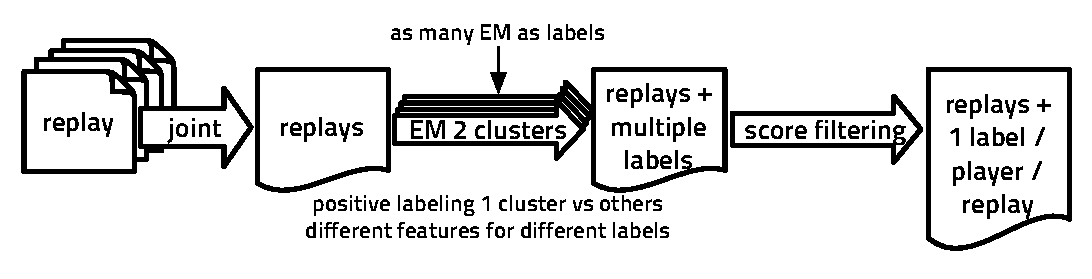
\includegraphics[width=1.0\columnwidth]{images/replays_labeling.pdf}}
\caption{Data centric view of our semi-supervised labeling of replays}
\label{replays_labeling}
\end{figure}

The selection of the features along with the opening labels is the supervised part of our labeling method. The knowledge of the features and openings comes from expert play and the StarCraft liquipedia\footnote{\url{http://wiki.teamliquid.net/starcraft/}}. They are all presented in Table~\ref{labels}. For instance, if we want to find out which replays correspond to the ``fast Dark Templar'' (DT, Protoss invisible unit) opening, we put the time at which the first Dark Templar is constructed as a feature and perform clustering on replays with it. This is what is needed for our playing bot: to be able to know when he has to fear ``fast DT'' opening and build a detector unit quickly to be able to deal with invisibility.


For the clustering part, we tried k-means, expectation-maximization (EM) with equal shape (bivariate normal distribution with proportional covariances matrices) and EM with the normal distribution shapes and volumes chosen with a Bayesian information criterion (BIC). Best BIC models were almost always the most agreeing with expert knowledge (15/17 labels). We used the R package Mclust \citep{Mclust,Mclust2} to perform full EM clustering. We produce ``2 bins clustering'' for each set of features (corresponding to each opening), and label the replays belonging to the cluster with the lower norm of features' appearances (that is exactly the purpose of our features). Figures~\ref{PvPspeedzeal} %\ref{TvZraxFE}
and \ref{ZvPmutas} show the clusters out of EM with the features of the corresponding openings. We thought of clustering because there are two cases in which you build a specific military unit of research a specific upgrade: either it is part of your opening, or it is part of your longer term game plan or even in reaction to the opponent. So the distribution over the time at which a feature appears is bimodal, with one (sharp) mode corresponding to ``opening with it'' and the other for the rest of the games, as can be seen in Figure~\ref{PvTfastDT}.

\begin{table*}[ht] \caption{Opening/Strategies labels of the replays (Weber's and ours are not always corresponding)}
\vspace{-0.5cm}
\begin{footnotesize}
\begin{center}
\begin{tabular}{|c|c|ccc|}
\hline
Race
& Weber's labels
& Our labels
& Features 
& Note (what we fear) \\ \hline
Protoss & FastLegs & speedzeal & Legs, GroundWeapons+1 & quick speed+upgrade attack\\
 & FastDT & fast\_dt & DarkTemplar & invisible units\\
 & FastObs & nony & Goon, Range & quick long ranged attack\\
 & ReaverDrop & reaver\_drop & Reaver, Shuttle & tactical attack zone damages \\
 & Carrier & corsair & Corsair & flying units \\
 & FastExpand & templar & Storm, Templar & powerful zone attack \\
 &  & two\_gates & 2ndGateway, Gateway, Zealot & aggressive rush \\
 & Unknown & unknown & (no clear label) & \\ \hline
Terran  & Bio & bio & 3rdBarracks, 2ndBarracks, Barracks & aggressive rush\\ 
 & TwoFactory & two\_facto & 2ndFactory & strong push (long range) \\ 
 & VultureHarass & vultures & Mines, Vulture & aggressive harass, invisible\\ 
 & SiegeExpand & fast\_exp & Expansion, Barracks & economical advantage \\ 
 & Standard & & & \\ 
 & FastDropship & drop & DropShip & tactical attack \\ 
 & Unknown & unknown & (no clear label) & \\ \hline
Zerg & TwoHatchMuta & fast\_mutas & Mutalisk, Gas & early air raid \\
 & ThreeHatchMuta & mutas & 3rdHatch, Mutalisk & massive air raid \\
 & HydraRush & hydras & Hydra, HydraSpeed, HydraRange & quick ranged attack\\
 & Standard & (speedlings) & (ZerglingSpeed, Zergling) & (removed, quick attacks/mobility) \\
 & HydraMass & & & \\
 & Lurker & lurkers & Lurker & invisible and zone damages \\
 & Unknown & unknown & (no clear label) & \\ \hline
\end{tabular}
\label{labels}
\end{center}
\end{footnotesize}
\end{table*}

\begin{table}[h]
\caption{Openings distributions for Terran in all the match-ups}
\vspace{-0.5cm}
\begin{center}
\begin{tabular}{|c|cc|cc|cc|}
\hline
&  & vs Protoss &  & vs Terran &  & vs Zerg \\
Opening
& Nb
& \begin{scriptsize}Percentage\end{scriptsize}
& Nb
& \begin{scriptsize}Percentage\end{scriptsize}
& Nb
& \begin{scriptsize}Percentage\end{scriptsize} \\ \hline
%%%two\_gates & 332 & & 252 & & 304 & \\
%%%fast\_dt & 7 & & 87 & & 20 & \\
%%%templar & 3 & & 17 & & 22 & \\
% TvP 1007
% TvT 576
% TvZ 872
bio 	    & 62 	& 6.2 	& 25 	& 4.4   & 197 	& 22.6 \\
fast\_exp 	& 438 	& 43.5 	& 377 	& 65.4  & 392 	& 44.9 \\
two\_facto 	& 240 	& 23.8  & 127 	& 22.0  & 116 	& 13.3 \\
vultures 	& 122 	& 12.1  & 3 	& 0.6   & 3 	& 0.3  \\
drop 	    & 52 	& 5.2   & 10 	& 1.7   & 121 	& 13.9 \\
unknown 	& 93 	& 9.3   & 34 	& 5.9   & 43 	& 5.0 \\ \hline
\end{tabular}
\label{openings_distrib}
\end{center}
\end{table}

\begin{figure}[htp]
\centerline{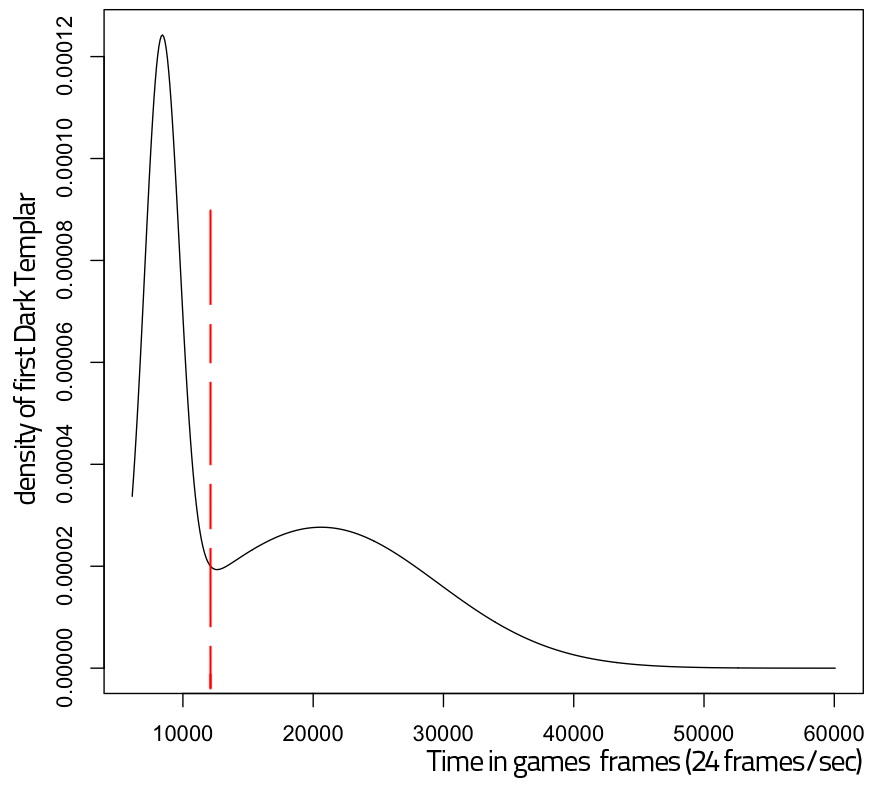
\includegraphics[width=0.7\columnwidth]{images/PvTfastDT.png}}
\caption{Protoss vs Terran distribution of first appearance of Dark Templars (Protoss invisible unit).}
\label{PvTfastDT}
\end{figure}

\begin{figure}[htp]
\centerline{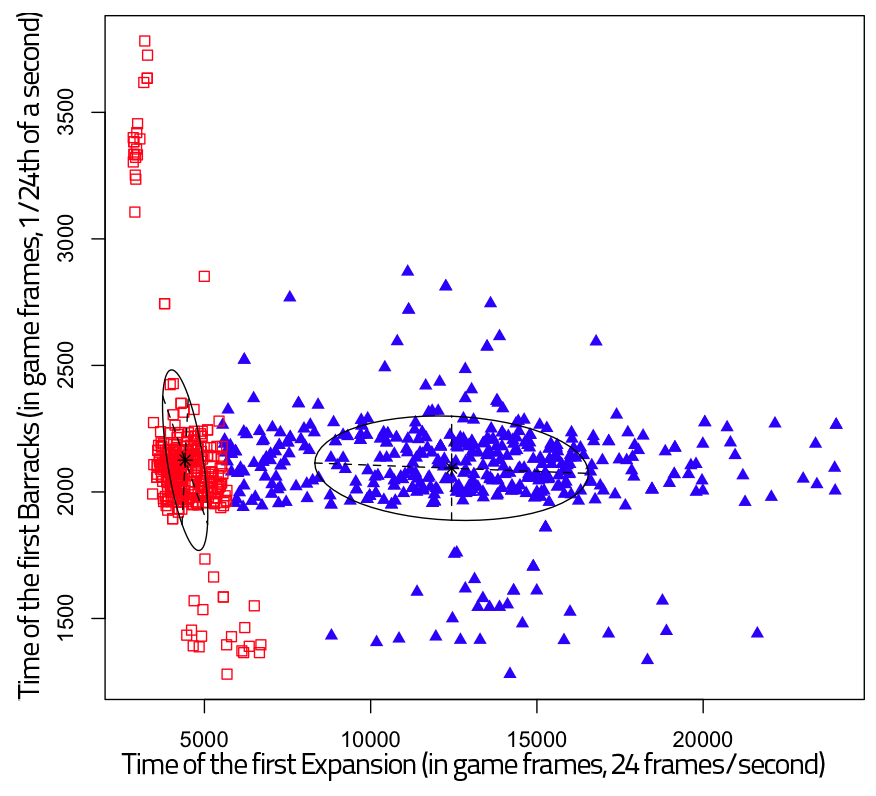
\includegraphics[width=0.9\columnwidth]{images/TvZraxFE.png}}
\caption{Terran vs Zerg Barracks and first Expansion timings (Terran). The bottom left cluster (squares) is the one labeled as \textit{fast\_exp}.}
\label{TvZraxFE}
\end{figure}

\begin{figure}[htp]
\centerline{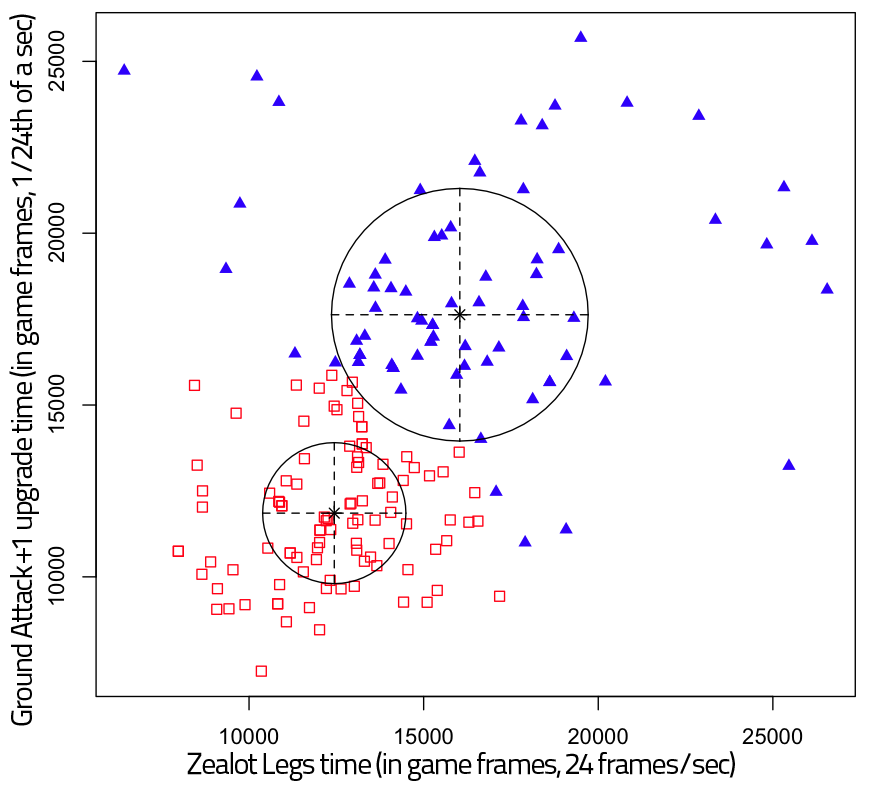
\includegraphics[width=0.9\columnwidth]{images/PvPspeedzeal.png}}
\caption{Protoss vs Protoss Ground Attack +1 and Zealot Legs upgrades timings. The bottom left cluster (squares) is the one labeled as \textit{speedzeal}.}
\label{PvPspeedzeal}
\end{figure}

\begin{figure}[htp]
\centerline{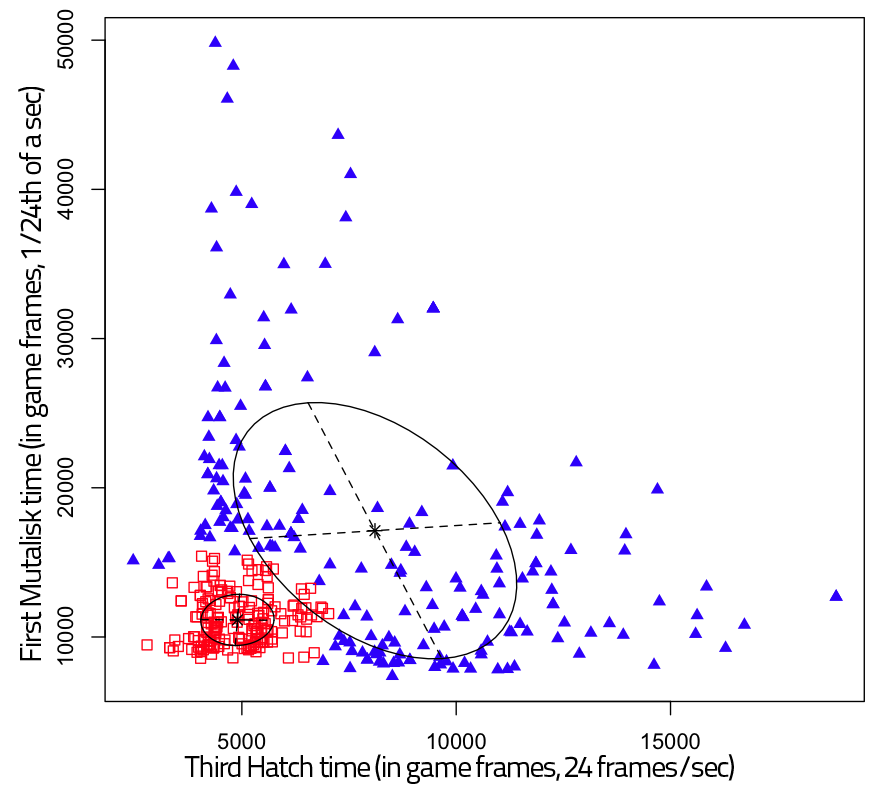
\includegraphics[width=0.9\columnwidth]{images/ZvPmutas.png}}
\vspace{-0.5cm}
\caption{Zerg vs Protoss time of the third Hatch and first appearance of Mutalisks. The bottom left cluster (squares) is the one labeled as \textit{mutas}.}
\label{ZvPmutas}
\end{figure}

Finally, some replays are labeled two or three times with different labels (due to the different time of effect of different openings), so we apply a filtering to transform multiple label replays into unique label ones (see Figure~\ref{replays_labeling}). For that we choose the openings labels that were happening the earliest (as they are a closer threat to the bot in a game setup) if and only if they were also the most probable or at 10\% of probability of the most probable label (to exclude transition boundaries of clusters) for this replay. We find the earliest by comparing the norms of the clusters means in competition. All replays without a label or with multiple labels (\textit{i.e.} which did not had a unique solution in filtering) after the filtering were labeled as \textit{unknown}. We then used this labeled dataset as well as Weber and Mateas' labels in the testing of our Bayesian model for opening prediction.

\subsection{Opening Prediction Model}

Our predictive model is a Bayesian program, it can be seen as the ``Bayesian network'' represented in Figure~\ref{BNPrediction}. It is a generative model and this is of great help to deal with the parts of the observations' space where we do not have too much data (RTS games tend to diverge from one another as the number of possible actions grow exponentially). Indeed, we can model our uncertainty by putting a large standard deviation on too rare observations and generative models tend to converge with fewer observations than discriminative ones \citep{Jordan}. Here is the description of our Bayesian program:

\begin{figure}[htp]
\centerline{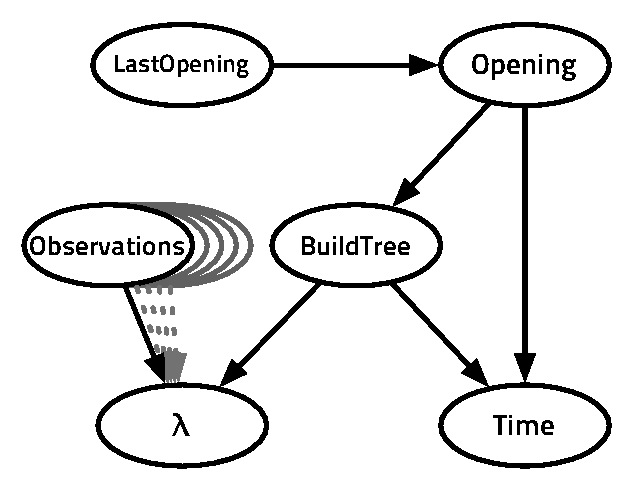
\includegraphics[width=0.6\columnwidth]{images/OpeningPrediction2.pdf}}
\caption{Graph representation of the opening (and tech tree) prediction model}
\label{BNPrediction}
\end{figure}

\subsubsection{Variables}
\begin{itemize}
\item $BuildTree \in [\emptyset, building_1, building_2, building_1\wedge building_2, techtrees, \dots]$: all the possible building trees for the given race. For instance $\{pylon, gate\}$ and $\{pylon, gate, core\}$ are two different $BuildTrees$.
\item $N\ Observations$: $O_{i \in \llbracket 1\dots N \rrbracket} \in \{0, 1\}$, $O_k$ is $1\ (true)$ if we have seen (observed) the $k$th building (it can have been destroyed, it will stay ``seen'').
\item $Opening$: $Op^t \in [opening_1 \dots opening_M]$ take the various opening values (depending on the race).
\item $LastOpening$: $Op^{t-1} \in [opening_1 \dots opening_M]$, Opening value of the previous time step (allows filtering, taking previous inference into account).
\item $\lambda \in \{0, 1\}$: coherence variable (restraining $BuildTree$ to possible values with regard to $O_\llbracket 1 \dots N \rrbracket$)
\item $Time$: $T \in \llbracket 1\dots P \rrbracket$, time in the game (1 second resolution).
\end{itemize}

At first, we generated all the possible (according to the game rules) $BuildTree$ values (between $\approx 500$ and $1600$ depending on the race). We observed that a lot of possible $BuildTree$ values are too absurd to be performed in a competitive match and were never seen during the learning. So, we restricted $BuildTree$ to have its value in all the build trees encountered in our replays dataset. 
%%%There are 292 build trees for Terran, 176 for Protoss and 113 for Zerg ($\approx 3000$ replays/race), all learned from the (unlabeled) replays.
There are 810 build trees for Terran, 346 for Protoss and 261 for Zerg ($\approx 3000$ replays/race), all learned from the (unlabeled) replays.

\subsubsection{Decomposition}
The joint distribution of our model is the following:
\begin{eqnarray*}
    & & P(T, BuildTree, O_1 \dots O_N, Op^t, Op^{t-1}, \lambda) \\ 
& = &   P(Op^t | Op^{t-1}) \\
    & & P(Op^{t-1}) \\
    & & P(BuildTree | Op^t) \\
    & & P(O_{\llbracket 1 \dots N\rrbracket}) \\
    & & P(\lambda | BuildTree, O_{\llbracket 1 \dots N\rrbracket}) \\
    & & P(T | BuildTree, Op^t) 
\end{eqnarray*}
This can also be see as Figure~\ref{BNPrediction}.

\subsubsection{Forms}
\begin{itemize}
\item $P(Op^t | Op^{t-1})$ is optional, we use it as a filter so that the previous inference impacts the current one. We use a functional Dirac:
\begin{eqnarray*}
& & P(Op^t|Op^{t-1})\ \  (Dirac)\\
& = & 1\ \mathrm{if}\ Op^t = Op^{t-1}\\
& = & 0\ \mathrm{else}
\end{eqnarray*}
This does not prevent our model to switch predictions, it just uses previous inference posterior $P(Op^{t-1}$ to average $P(Op^t)$.

\item $P(Op^{t-1})$ copied from one inference to another (mutated from $P(Op^t)$). The first $P(Op^{t-1})$ is bootstrapped with the uniform distribution, we could also use a prior on openings in the given match-up.
\item $P(BuildTree | Op^t)$ is learned from the labeled replays. $P(BuildTree|Op^t)$ are $\mathrm{card}(\{openings\})$ different histogram over the values of $BuildTree$.
\item $P(O_{\llbracket 1 \dots N\rrbracket})$ is unspecified, we put the uniform distribution (we could use a prior over the most frequent observations).
\item $P(\lambda | BuildTree, O_{\llbracket 1 \dots N\rrbracket})$ is a functional Dirac that restricts $BuildTree$ values to the ones than can co-exist with the observations.
\begin{eqnarray*}
& & P(\lambda = 1 | buildTree, o_{\llbracket 1 \dots N\rrbracket}) \\
& = & 1\ \mathrm{if\ } buildTree \ \mathrm{can\ exist\ with\ } o_{\llbracket 1\dots N\rrbracket} \\
& = & 0\ \mathrm{else}
\end{eqnarray*}
A $BuildTree$ value ($buildTree$) is compatible with the observations if it covers them fully. For instance, $BuildTree=\{pylon, gate, core\}$ is compatible with $o_{\#core} = 1$ but it is not compatible with $o_{\#forge} = 1$. In other words, $buildTree$ is incompatible with $o_{\llbracket 1\dots N\rrbracket}$ \textit{iff} $\{o_{\llbracket 1\dots N\rrbracket} \backslash \{o_{\llbracket 1\dots N\rrbracket} \wedge buildTree\}\} \neq \emptyset$.
\item $P(T | BuildTree, Op^t)$ are ``bell shape'' distributions (discretized normal distributions). There is one bell shape per couple $(opening, buildTree)$. The parameters of these discrete Gaussian distributions are learned from the labeled replays.
\end{itemize}

\subsubsection{Identification (learning)}
The learning of the $P(BuildTree | Op^t)$ histogram is straight forward counting of occurrences from the labeled replays. The learning of the $P(T | BuildTree, Op^t)$ bell shapes parameters takes into account the uncertainty of the couples $(buildTree, opening)$ for which we have few observations. Indeed, the normal distribution $P(T|buildTree, opening)$ begins with a high $\sigma^2$, and \textbf{not} a Dirac with $\mu$ on the seen $T$ value and $sigma=0$. This accounts for the fact that the first observation may have been an outlier. This learning process is independent on the order of the stream of examples, seeing point A and then B or B and then A in the learning phase produces the same result. 

\begin{figure}[htp]
\centerline{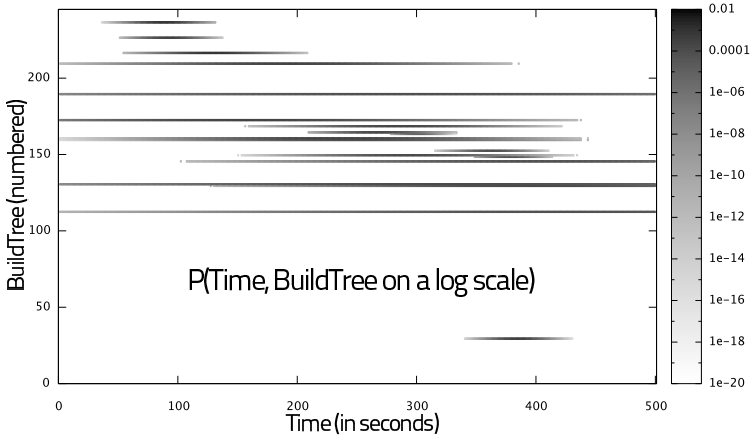
\includegraphics[width=1.0\columnwidth]{images/BW_HeatMap_knowing_ReaverDrop.png}}
\caption{$P(Time, BuildTree | Opening^t=ReaverDrop)$}
\label{noise}
\end{figure}


\subsubsection{Questions}
%%%\begin{eqnarray*}
%%%P(Op|T=t, O_{1:N}=o_{1:N}, \lambda = 1) \\
%%%\propto \frac{1} {P(o_{1:N}).P(\lambda).P(t)} \\
%%%\sum_{BuildTree} P(Op).P(BuildTree|Op).P(o_{1:N})\\
%%%.P(\lambda|BuildTree,o_{1:N}).P(t|BuildTree,Op)
%%%\end{eqnarray*}
The question that we will ask in all the benchmarks is:
\begin{eqnarray*}
 & P(Op|T=t, O_{\llbracket 1\dots N\rrbracket}=o_{\llbracket 1\dots N\rrbracket}, \lambda = 1) \\
 & \propto P(Op).P(o_{\llbracket 1\dots N\rrbracket})\\
 & \times \sum_{BuildTree} P(\lambda | BuildTree, o_{\llbracket 1\dots N\rrbracket})\\
 & .P(BuildTree|Op).P(t|BuildTree, Op)
\end{eqnarray*}
Note that if we see $P(BuildTree, Time)$ as a plan, asking $P(BuildTree|Opening, Time)$ boils down to use our ``plan recognition'' mode as a planning algorithm, which could provide good approximations of the optimal goal set \citep{Ramirez}. This gives us a distribution on the build trees to follow (build orders) to achieve a given opening.

\subsection{Results on StarCraft}

\subsubsection{Prediction}

For each match-up, we ran cross-validation testing with 9/10th of the dataset used for learning and the remaining 1/10th of the dataset used for testing. We ran tests finishing at 5, 10 and 15 minutes to capture all kinds of openings (early to late ones). To measure the predictive capability of our model, we used 3 metrics: 
\begin{itemize}
\item the \textit{final} prediction, which is the opening that is predicted at the end of the test, 
\item the \textit{online twice} (OT), which counts the openings that have emerged as most probable twice a test (so that their predominance is not due to noise),
\item the \textit{online once} $> 3$ (OO3), which counts the openings that have emerged as most probable openings after 3 minutes (so that these predictions are based on really meaningful information).
\end{itemize}
After 3 minutes, a Terran player will have or be building his first supply depot, barracks, refinery (gas), and at least factory or expansion. A Zerg player would have his first overlord, zergling pool, extractor (gas) and most of the time his expansion and lair tech. A Protoss player would have his first pylon, gateway, assimilator (gas), cybernectics core, and sometimes his robotics center, or forge and expansion.

\begin{figure}[htp]
\centerline{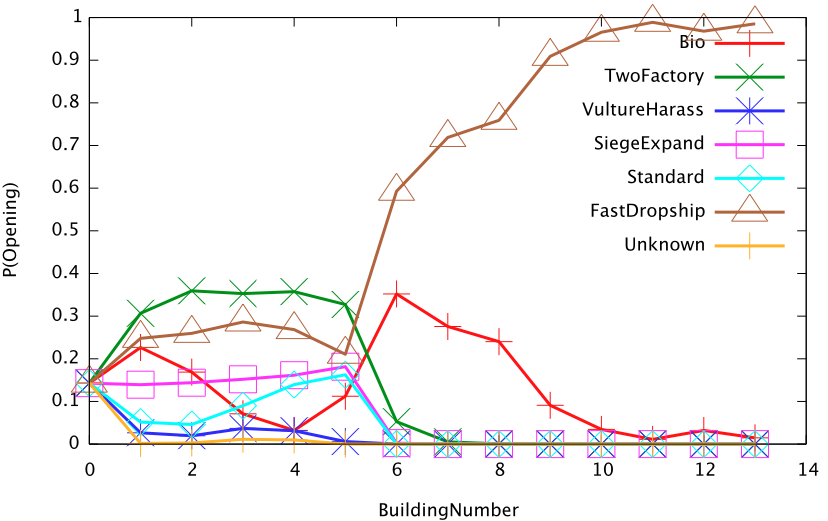
\includegraphics[width=1.0\columnwidth]{images/TvP_prediction.png}}
\vspace{-0.2cm}
\centerline{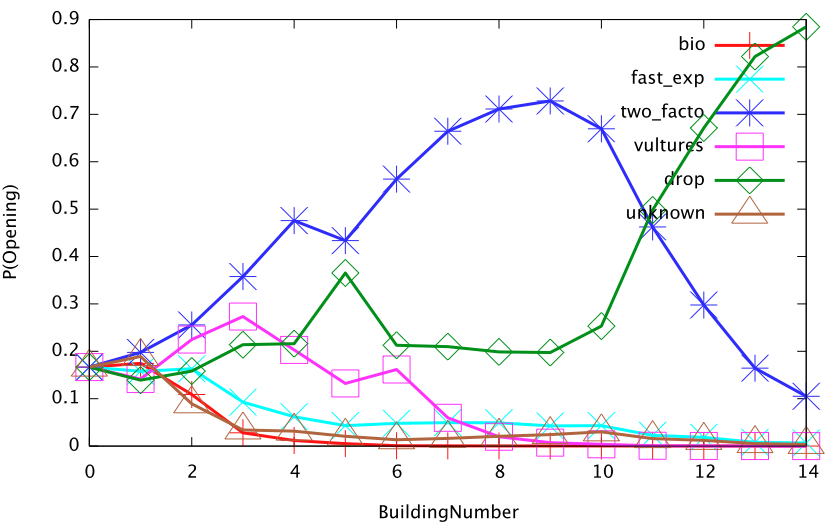
\includegraphics[width=1.0\columnwidth]{images/TvPx_prediction.png}}
\vspace{-0.3cm}
\caption{Evolution of $P(Opening)$ with increasing observations in a TvP match-up, with Weber's labeling on top, our labeling on the bottom. The x-axis corresponds to the construction of buildings.}
\label{prediction}
\vspace{-0.5cm}
\end{figure}

Table~\ref{results} sums up all the prediction probabilities (scores) of our model in all the match-ups with both labeling of the game logs. Please note that when an opening is mispredicted, the distribution on openings is often not $P(badopening)=1, P(others)=0$ and that we can extract some value out of these distributions. Also, we observed that $P(Opening=unknown)>P(others)$ is often a case of misprediction: our bot would use the next prediction in this case. Figure~\ref{prediction} shows the evolution of the distribution $P(Opening)$ during a replay for Weber's and our labelings. Figure~\ref{noise} shows the resistance of our model to noise. We randomly removed some observations (buildings, attributes), from 1 to 15, knowing that for Protoss and Terran we use 16 buildings observations and 17 for Zerg. We think that our model copes well with noise because it backtracks unseen observations: for instance if we have only the $core$ observation, it will work with build trees containing $core$ that will passively infer unseen $pylon$ and $gate$. Also, uncertainty is handled natively.



\begin{figure}[htp]
\centerline{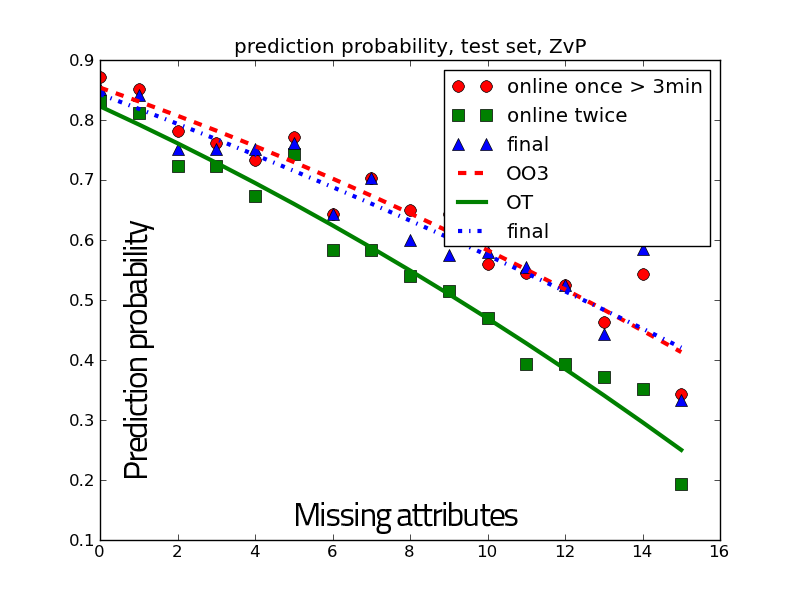
\includegraphics[width=1.0\columnwidth]{images/ZvP2.png}}
\vspace{-0.2cm}
\centerline{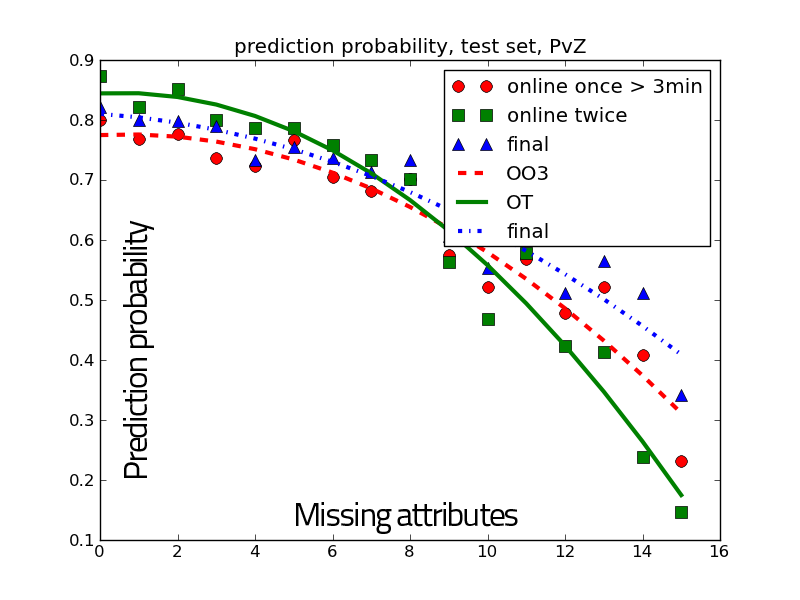
\includegraphics[width=1.0\columnwidth]{images/PvZ2.png}}
\vspace{-0.3cm}
\caption{Two extreme evolutions of the 3 probabilities of opening recognition with increasing noise (15 missing attributes/observations/buildings correspond to 93.75\% missing information for Protoss and Terran openings prediction and 88.23\% of missing attributes for Zerg openings prediction). Zerg opening prediction probabilitly on top, Protoss bottom.}
\label{noise}
\end{figure}

\begin{table*}[ht] \caption{Prediction probabilities for all the match-ups}
\vspace{-0.5cm}
\begin{center}
\begin{tabular}{|c|ccc|ccc|ccc|ccc|ccc|ccc|}
\hline
& \multicolumn{9}{|c|}{Weber and Mateas' labels}
& \multicolumn{9}{|c|}{Our labels}
\\  \hline
& \multicolumn{3}{|c|}{5 minutes}
& \multicolumn{3}{|c|}{10 minutes}
& \multicolumn{3}{|c|}{15 minutes}
& \multicolumn{3}{|c|}{5 minutes}
& \multicolumn{3}{|c|}{10 minutes}
& \multicolumn{3}{|c|}{15 minutes}
\\
\begin{scriptsize}match-up\end{scriptsize}
& final
& OT
& OO3
& final
& OT
& OO3
& final
& OT
& OO3
& final
& OT
& OO3
& final
& OT
& OO3
& final
& OT
& OO3 \\ \hline
PvP & 0.65 & 0.53 & 0.59 & 0.69 & 0.69 & 0.71 & 0.65 & 0.67 & 0.73
& 0.78 & 0.74 & 0.68 & 0.83 & 0.83 & 0.83 & 0.85 & 0.83 & 0.83 \\
PvT & 0.75 & 0.64 & 0.71 & 0.78 & 0.86 & 0.83 & 0.81 & 0.88 & 0.84
& 0.62 & 0.69 & 0.69 & 0.62 & 0.73 & 0.72 & 0.6 & 0.79 & 0.76 \\
PvZ & 0.73 & 0.71 & 0.66 & 0.8 & 0.86 & 0.8 & 0.82 & 0.87 & 0.8
& 0.61 & 0.6 & 0.62 & 0.66 & 0.66 & 0.69 & 0.61 & 0.62 & 0.62 \\
TvP & 0.69 & 0.63 & 0.76 & 0.6 & 0.75 & 0.77 & 0.55 & 0.73 & 0.75
& 0.50 & 0.47 & 0.54 & 0.5 & 0.6 & 0.69 & 0.42 & 0.62 & 0.65 \\
TvT & 0.57 & 0.55 & 0.65 & 0.5 & 0.55 & 0.62 & 0.4 & 0.52 & 0.58
& 0.72 & 0.75 & 0.77 & 0.68 & 0.89 & 0.84 & 0.7 & 0.88 & 0.8 \\
TvZ & 0.84 & 0.82 & 0.81 & 0.88 & 0.91 & 0.93 & 0.89 & 0.91 & 0.93
& 0.71 & 0.78 & 0.77 & 0.72 & 0.88 & 0.86 & 0.68 & 0.82 & 0.81 \\
ZvP & 0.63 & 0.59 & 0.64 & 0.87 & 0.82 & 0.89 & 0.85 & 0.83 & 0.87
& 0.39 & 0.56 & 0.52 & 0.35 & 0.6 & 0.57 & 0.41 & 0.61 & 0.62 \\
ZvT & 0.59 & 0.51 & 0.59 & 0.68 & 0.69 & 0.72 & 0.57 & 0.68 & 0.7
& 0.54 & 0.63 & 0.61 & 0.52 & 0.67 & 0.62 & 0.55 & 0.73 & 0.66 \\
ZvZ & 0.69 & 0.64 & 0.67 & 0.73 & 0.74 & 0.77 & 0.7 & 0.73 & 0.73
& 0.83 & 0.85 & 0.85 & 0.81 & 0.89 & 0.94 & 0.81 &  0.88 & 0.94\\ \hline
\begin{scriptsize}overall\end{scriptsize} & 0.68 & 0.62 & 0.68 & 0.73 & 0.76 & 0.78 & 0.69 & 0.76 & 0.77 
& 0.63 & 0.67 & 0.67 & 0.63 & 0.75 & 0.75 & 0.63 & 0.75 & 0.74 \\ \hline
\end{tabular}
\label{results}
\end{center}
\end{table*}


\subsubsection{Performances}
The first iteration of this model was not making use of the structure imposed by the game in the form of ``possible build trees'' and was at best very slow, at worst intractable without sampling. With the model presented here, the performances are ready for production as shown in Table~\ref{CPU}. The memory footprint is around 3.5Mb on a 64bits machine. Learning computation time is linear in the number of games logs events ($O(N)$ with $N$ observations), which are bounded, so it is linear in the number of game logs. It can be serialized and done only once when the dataset changes. The prediction computation corresponds to the sum in the question (III.B.5) and so its computational complexity is in $O(N\cdot M)$ with $N$ build trees and $M$ possible observations, as $M << N$, we can consider it linear in the number of build trees (values of $BuildTree$).

\begin{table}[h]
\caption{Extremes of computation time values (in seconds, C2D 2.8Ghz)}
\vspace{-0.5cm}
\begin{center}
\begin{tabular}{|c|cc|cc|}
\hline
Race
& Nb Games
& Learning time
& Inference $\mu$
& Inference $\sigma^2$ \\ \hline
T (max) & 1036 & 0.197844 & 0.0360234 & 0.00892601 \\
T \begin{tiny}(Terran)\end{tiny} & 567 & 0.110019 & 0.030129 & 0.00738386 \\ 
P \begin{tiny}(Protoss)\end{tiny} & 1021 & 0.13513 & 0.0164457 & 0.00370478 \\
P \begin{tiny}(Protoss)\end{tiny} & 542 & 0.056275 & 0.00940027 & 0.00188217 \\ 
Z \begin{tiny}(Zerg)\end{tiny} & 1028 & 0.143851 & 0.0150968 & 0.00334057 \\
Z \begin{tiny}(Zerg)\end{tiny} & 896 & 0.089014 & 0.00796715 & 0.00123551 \\ \hline
\end{tabular}
\label{CPU}
\end{center}
\end{table}

\subsection{Extensions}

\subsubsection{Possible Uses}
Developing beforehand a RTS game AI that specifically deals with whatever strategies the players will come up is very hard. And even if game developers were willing to patch their AI afterwards, it would require a really modular design and a lot of work to treat each strategy. With our model, the AI can adapt to the evolutions in play by learning its parameters from the replay, and it can dynamically adapt during the games by using the reverse question $P(BuildTree | Opening,Time)$, or even $P(TechTree | Opening, Time)$ if we use a $TechTree$ variable encoding buildings and technology upgrades. This question would give the distribution over technology trees knowing the opening we want to perform at which time. This would allow for the bot to dynamically choose/change build orders.

We could also use this model in a commentary assistant AI. In the StarCraft and StarCraft 2 communities, there are a lot of \gloss{pro-gamer} tournaments that are commented and we could provide a tool for commentators to estimate the probabilities or different openings or technology paths. As in commented poker matches, where the probabilities of different hands are drawn on screen for the spectators, we could display the probabilities of openings. In such a setup we could use more features as the observers and commentators can see everything that happens (upgrades, units) and we limited ourselves to ``key'' buildings in the work presented in this paper.

\subsubsection{Improvements}

First, our prediction model can be upgraded to have a higher recognition rate: we could reason about $t+1$ explicitly before computing the distribution over possible openings at $t$ and thus compute the distribution over technology trees at $t+1$. Perhaps it would increase the results of $P(Opening|Observations)$, but it almost surely would increase $P(BuildTree^{t+1}|Observations)$ which is important for late game predictions. We could also make use of more features as we currently only use at most 20 features (only buildings), and never all at once. Perhaps also that incorporating priors per match-up would lead to better results.

Then, we could feed it with \textit{more} replays during the learning by scrapping more progamers level replays websites. Also, we could learn from replays of bot vs bot matches. For the learning part, the labeling of replays is very important, and our labeling methods can be improved. 
We could explore auto-supervised learning \citep{AutoSuperLearning}. 
Clearly, some match-ups are handled better, either in the replays labeling part and/or in the prediction part. Replays could be labeled by humans and we would do supervised learning then. Or they could be labeled by a combination of rules (as in \citep{weber}) and statistical analysis (as the method presented here). Finally, the replays could be labeled by match-up dependent openings (instead of race dependent openings currently) and could contain either the two parts of the opening %(early and late developments) 
or the game time at which the label is the most relevant, as openings are often bimodal (``fast expand into mutas'', ``corsairs into reaver'', etc.).

Finally, a hard problem is detecting the ``fake'' builds of very highly skilled players. Indeed, some progamers have build orders which purpose are to fool the opponent into thinking that they are performing opening A while they are doing B. %For instance they could ``take early gas'' leading the opponent to think they are going to do tech units, not gather gas 
For instance, they could leadthe opponent to think they are going to \textit{tech} 
and perform an early rush instead. We think that this can be handled by our model by changing $P(Opening|LastOpening)$ by $P(Opening|LastOpening, LastObservations)$ and adapting the influence of the last prediction with regard to the last observations (i.e., we think we can learn some ``fake'' label on replays).

\section{Strategy adaptation}

\subsection{Related Works}
\subsection{Strategy Adaptation Model}
\subsection{Results on StarCraft}
\subsection{Extensions}





